%\documentclass{standalone}
\documentclass{article}
\usepackage{tikz}
\usepackage{amsmath}
\begin{document}
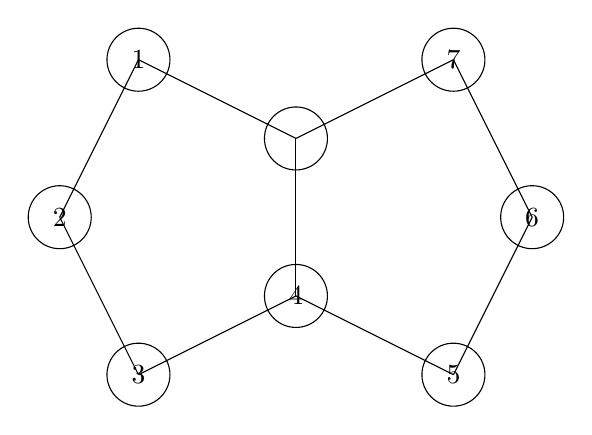
\begin{tikzpicture}[scale=1]
  \def\r{.4}
  \draw (-2, 3) circle [radius=\r] -- (-3, 1)circle [radius=\r] -- (-2, -1) circle [radius=\r] -- (0, 0) circle [radius=\r] -- (2, -1) circle [radius=\r] -- (3, 1) circle [radius=\r] -- (2, 3) circle [radius=\r] -- (0, 2) circle [radius=\r] -- (-2, 3);
  \draw (0,0) -- (0, 2);
  \foreach \i/\x/\y in {1/-2/3, 2/-3/1, 3/-2/-1, 4/0/0, 5/2/-1, 6/3/1, 7/2/3} {
    \draw (\x, \y) node{\i};
  }
\end{tikzpicture}
\end{document}
